\documentclass[12pt,letterpaper]{article}\usepackage[]{graphicx}\usepackage[]{color}
%% maxwidth is the original width if it is less than linewidth
%% otherwise use linewidth (to make sure the graphics do not exceed the margin)
\makeatletter
\def\maxwidth{ %
  \ifdim\Gin@nat@width>\linewidth
    \linewidth
  \else
    \Gin@nat@width
  \fi
}
\makeatother

\definecolor{fgcolor}{rgb}{0.345, 0.345, 0.345}
\newcommand{\hlnum}[1]{\textcolor[rgb]{0.686,0.059,0.569}{#1}}%
\newcommand{\hlstr}[1]{\textcolor[rgb]{0.192,0.494,0.8}{#1}}%
\newcommand{\hlcom}[1]{\textcolor[rgb]{0.678,0.584,0.686}{\textit{#1}}}%
\newcommand{\hlopt}[1]{\textcolor[rgb]{0,0,0}{#1}}%
\newcommand{\hlstd}[1]{\textcolor[rgb]{0.345,0.345,0.345}{#1}}%
\newcommand{\hlkwa}[1]{\textcolor[rgb]{0.161,0.373,0.58}{\textbf{#1}}}%
\newcommand{\hlkwb}[1]{\textcolor[rgb]{0.69,0.353,0.396}{#1}}%
\newcommand{\hlkwc}[1]{\textcolor[rgb]{0.333,0.667,0.333}{#1}}%
\newcommand{\hlkwd}[1]{\textcolor[rgb]{0.737,0.353,0.396}{\textbf{#1}}}%
\let\hlipl\hlkwb

\usepackage{framed}
\makeatletter
\newenvironment{kframe}{%
 \def\at@end@of@kframe{}%
 \ifinner\ifhmode%
  \def\at@end@of@kframe{\end{minipage}}%
  \begin{minipage}{\columnwidth}%
 \fi\fi%
 \def\FrameCommand##1{\hskip\@totalleftmargin \hskip-\fboxsep
 \colorbox{shadecolor}{##1}\hskip-\fboxsep
     % There is no \\@totalrightmargin, so:
     \hskip-\linewidth \hskip-\@totalleftmargin \hskip\columnwidth}%
 \MakeFramed {\advance\hsize-\width
   \@totalleftmargin\z@ \linewidth\hsize
   \@setminipage}}%
 {\par\unskip\endMakeFramed%
 \at@end@of@kframe}
\makeatother

\definecolor{shadecolor}{rgb}{.97, .97, .97}
\definecolor{messagecolor}{rgb}{0, 0, 0}
\definecolor{warningcolor}{rgb}{1, 0, 1}
\definecolor{errorcolor}{rgb}{1, 0, 0}
\newenvironment{knitrout}{}{} % an empty environment to be redefined in TeX

\usepackage{alltt}

\usepackage{amsmath}
\usepackage{bm} % for bold math symbols
\usepackage{booktabs} % better tables
\usepackage[left=.4in,right=.2in,top=.4in,bottom=.2in]{geometry} % margins
\usepackage{caption} % for subfigures
\usepackage[T1]{fontenc} % see http://goo.gl/KXXek
\usepackage{graphicx} % obviously for graphics
\usepackage{lscape}
\usepackage{listings} % source code
\usepackage{latexsym} % MBE template for some fonts
\usepackage{mathtools} % an extension to amsmath to fix bugs
\usepackage{multirow} % column cells that span multiple rows
\usepackage{natbib} % nicer references
\usepackage{paralist} % inline lists
\usepackage[section]{placeins} % keep figures and table inside section
\usepackage{setspace} % for line spacing
\usepackage{subfig} % for subfigures
\IfFileExists{upquote.sty}{\usepackage{upquote}}{}
\begin{document}



\section*{Data}
There are 35 taxa with 3738 codons (3539 without ambiguous sites) in the
concatenated alignment.  Each of the 10 branch-site tests is on a single branch.

\begin{figure}[h!]
  % \centering
\begin{knitrout}
\definecolor{shadecolor}{rgb}{0.969, 0.969, 0.969}\color{fgcolor}

{\centering 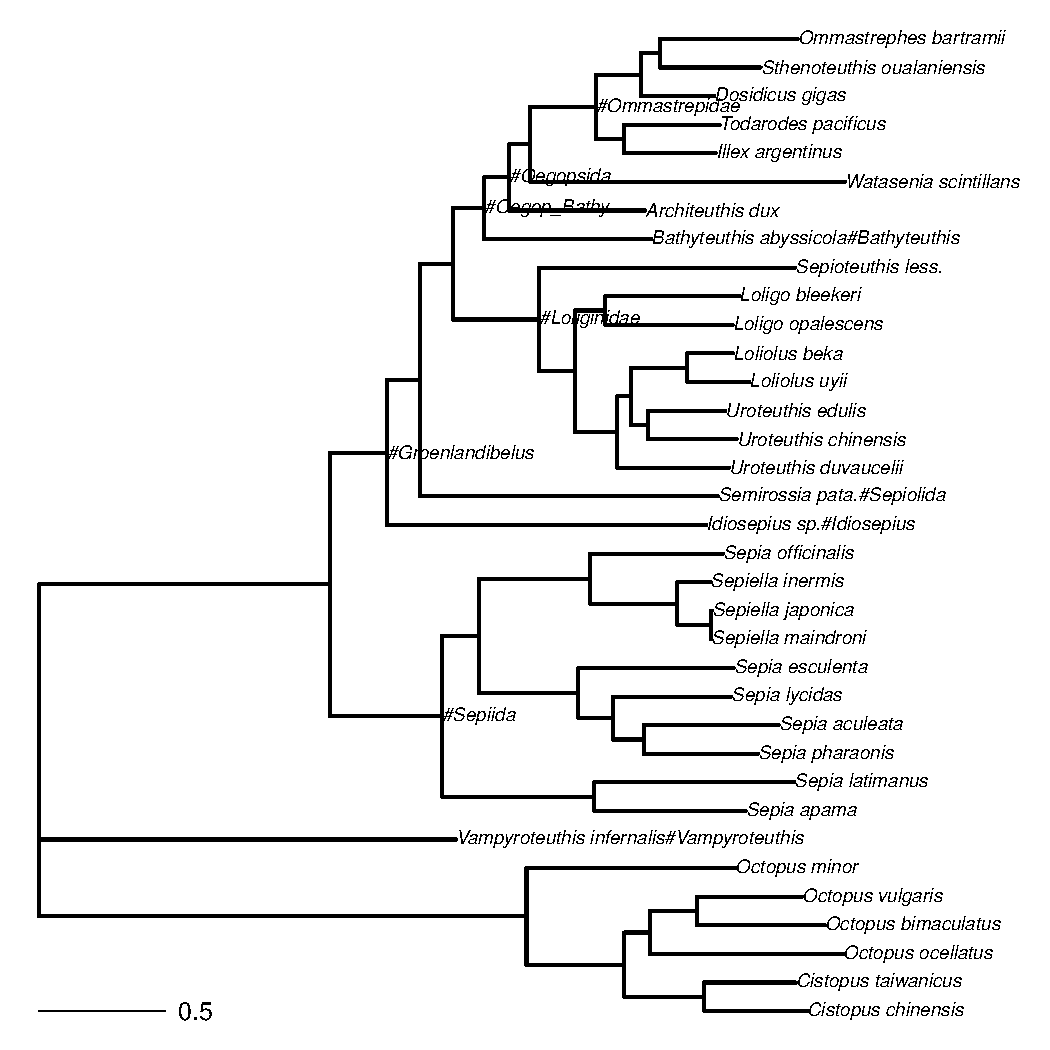
\includegraphics[width=\maxwidth]{./figures/tree-1} 

}



\end{knitrout}
  \caption[]{Tree labelled with each foreground branch tested under a branch-site model.}
  \label{fig:ceph_tree}
\end{figure}

\clearpage

\section*{Branch-Site Tests}
\begin{knitrout}
\definecolor{shadecolor}{rgb}{0.969, 0.969, 0.969}\color{fgcolor}\begin{table}[!h]

\caption{\label{tab:lr}Branch-site model likelihood ratio tests.  Correcting for
multiple tests does not change the results.  Tests along the Groenlandibelus,
Loliginidae, OegopBathy, Oegop\_Bathy, and Sepiida branches are significant.}
\centering
\begin{tabular}{lrrrr}
\toprule
Branch Tested & H0 & Ha & LRS & p-value\\
\midrule
Bathyteuthis & -156044.3 & -156044.3 & 0.000000 & 0.5000000\\
Groenlandibelus & -155990.8 & -155974.3 & 32.971196 & 0.0000000\\
Idiosepius & -156004.9 & -156004.7 & 0.332972 & 0.2819571\\
Loliginidae & -155953.6 & -155945.5 & 16.195108 & 0.0000286\\
Oegop\_Bathy & -156012.1 & -156005.1 & 14.102188 & 0.0000866\\
\addlinespace
Oegopsida & -156033.4 & -156028.6 & 9.690420 & 0.0009262\\
Ommastrepidae & -156027.4 & -156027.3 & 0.177430 & 0.3367956\\
Sepiida & -155926.7 & -155898.3 & 56.892882 & 0.0000000\\
Sepiolida & -156021.7 & -156021.7 & 0.000000 & 0.5000000\\
Vampyroteuthis & -156007.8 & -156007.8 & 0.000000 & 0.5000000\\
\bottomrule
\end{tabular}
\end{table}


\end{knitrout}

\clearpage

\section*{SBA MLE Distributions}
%SBA was run for the five significant branch-site tests.

% \begin{figure}[h!]
%   % \centering
%   <<tree-sig-foreground,echo=F,cache=F>>=
%   tree <- read.tree("../../data/Data_28May_2019_TE/ceph.tre");
%   plot(tree,no.margin=T,cex=0.75,type="phylogram",edge.width=2,lab4ut="axial",show.node.label=T)
%   add.scale.bar()
%   @
%   \caption[]{Tree with each foreground branch of interest labelled.}
%   \label{fig:ceph_tree}
% \end{figure}


\subsection*{Greonlandibelus}



\begin{knitrout}
\definecolor{shadecolor}{rgb}{0.969, 0.969, 0.969}\color{fgcolor}

{\centering 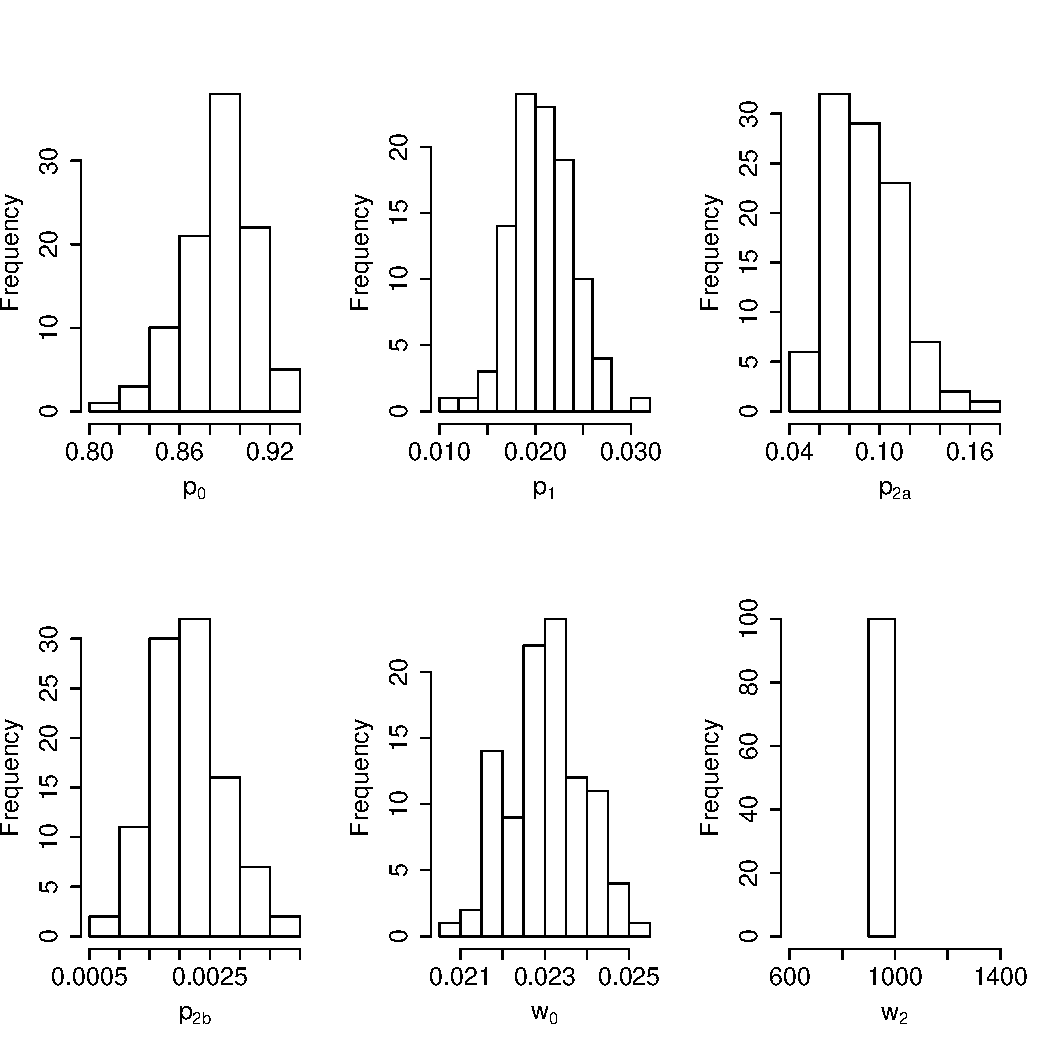
\includegraphics[width=\maxwidth]{./figures/Groenlandibelus_plots-1} 

}



\end{knitrout}

\clearpage

\subsection*{Loliginidae}


\begin{knitrout}
\definecolor{shadecolor}{rgb}{0.969, 0.969, 0.969}\color{fgcolor}

{\centering 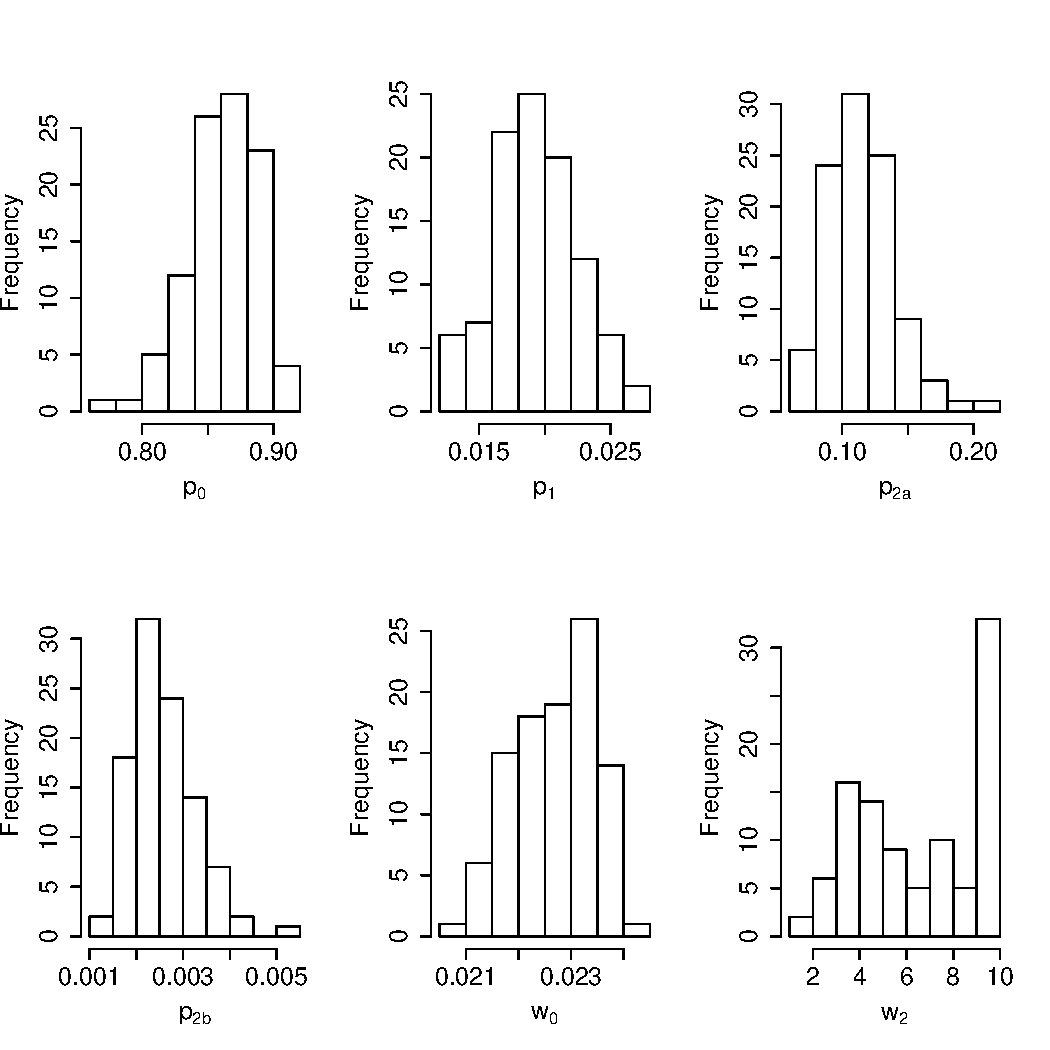
\includegraphics[width=\maxwidth]{./figures/Loliginidae_plots-1} 

}



\end{knitrout}

\clearpage

\subsection*{Oegop\_Bathy}


\begin{knitrout}
\definecolor{shadecolor}{rgb}{0.969, 0.969, 0.969}\color{fgcolor}

{\centering 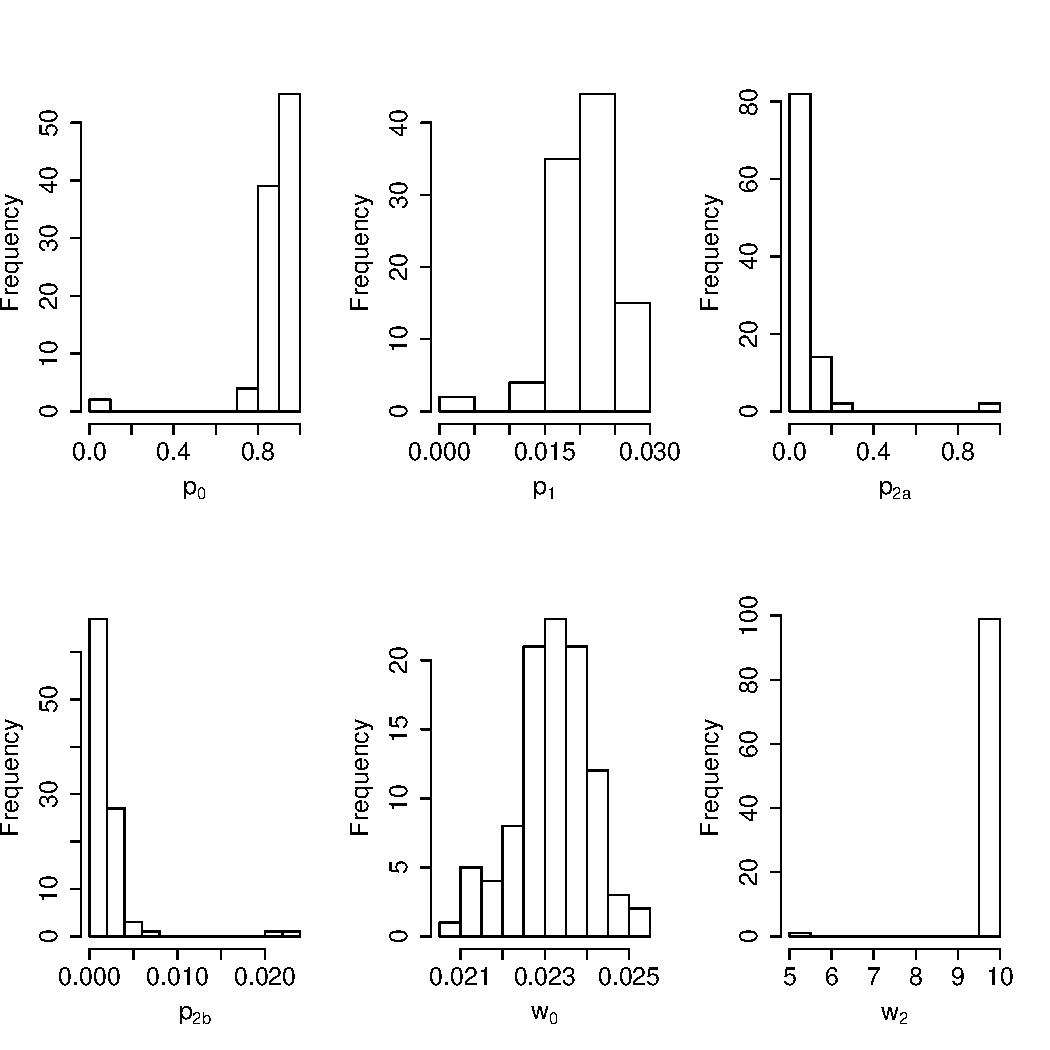
\includegraphics[width=\maxwidth]{./figures/OegopBathy_plots-1} 

}



\end{knitrout}

\clearpage

\subsection*{Oegopsida}


\begin{knitrout}
\definecolor{shadecolor}{rgb}{0.969, 0.969, 0.969}\color{fgcolor}

{\centering 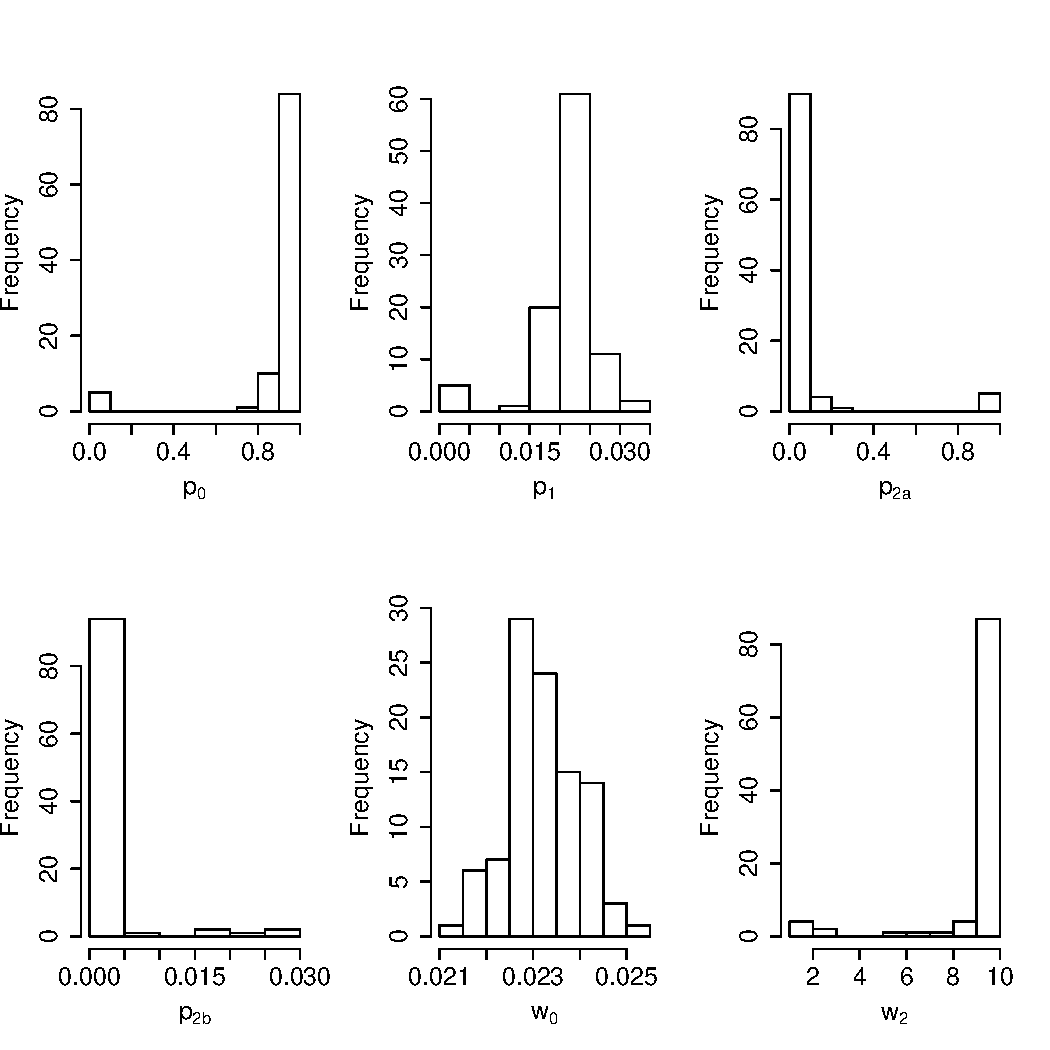
\includegraphics[width=\maxwidth]{./figures/Oegopsida_plots-1} 

}



\end{knitrout}

\clearpage

\subsection*{Sepiida}


\begin{knitrout}
\definecolor{shadecolor}{rgb}{0.969, 0.969, 0.969}\color{fgcolor}

{\centering 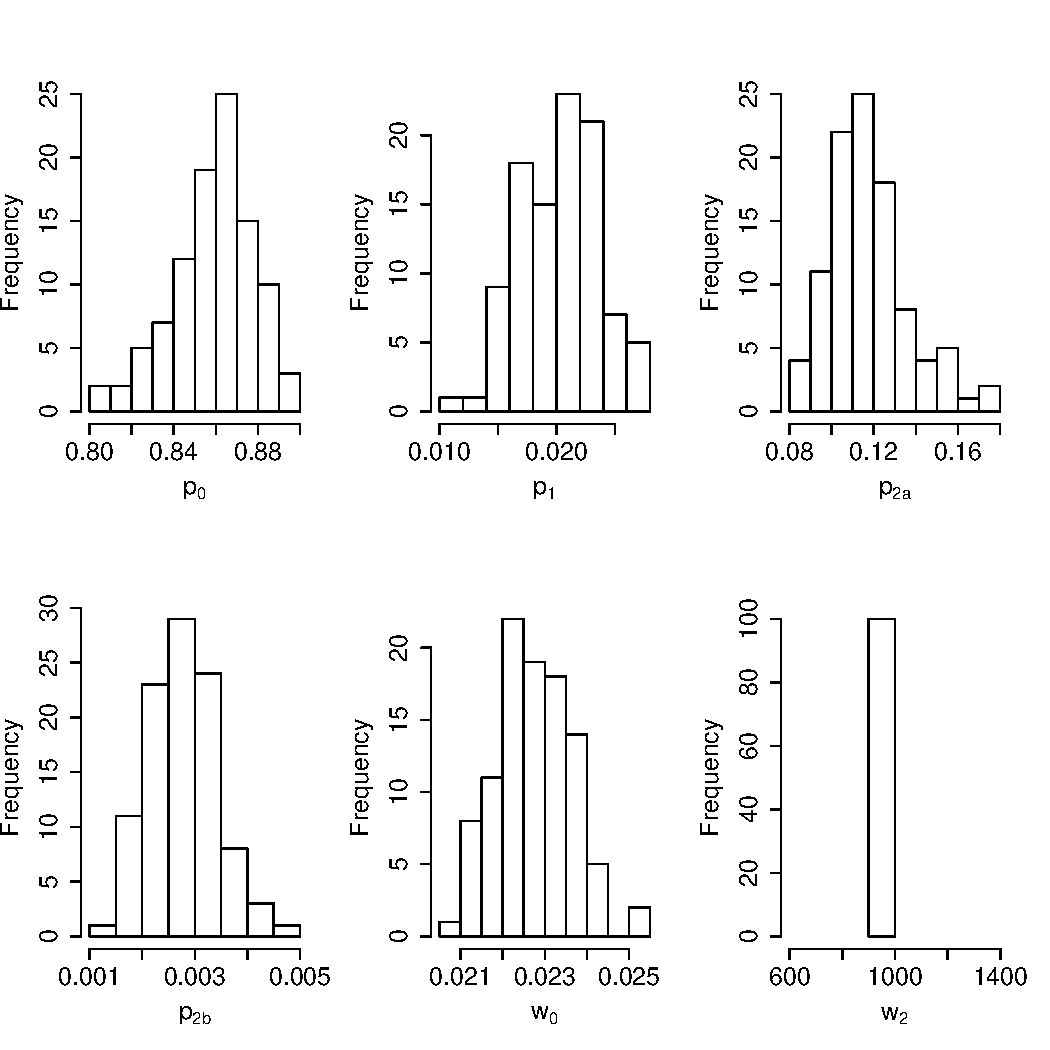
\includegraphics[width=\maxwidth]{./figures/Sepiida_plots-1} 

}



\end{knitrout}

\clearpage

\subsection*{Site Classification}

\begin{table}[!ht]
  \centering
  \begin{tabular}{*{10}l}
    \toprule
    & \multicolumn{3}{c}{BEB} & \multicolumn{3}{c}{SBA (mean)} & \multicolumn{3}{c}{SBA (median)}  \\
    \cmidrule(lr){2-4} \cmidrule(lr){5-7} \cmidrule(lr){8-10}
    Branch             & 0.5 & 0.95 & 0.99 & 0.5 & 0.95 & 0.99 & 0.5 & 0.95 & 0.99 \\
    \cmidrule(lr){1-1} \cmidrule(lr){2-2} \cmidrule(lr){3-3} \cmidrule(lr){4-4} \cmidrule(lr){5-5} \cmidrule(lr){6-6} \cmidrule(lr){7-7} \cmidrule(lr){8-8} \cmidrule(lr){9-9} \cmidrule(lr){10-10}
    Groenlandibelus    & 0   & 0    & 0   & 127  & 38   & 9    & 132 & 51   & 17   \\
    Loliginidae        & 163 & 19   & 13  & 141  & 12   & 7    & 143 & 86   & 12   \\
    Oegop\_Bathy       & 0   & 0    & 0   & 66   & 18   & 2    & 71  & 32   & 16   \\
    Oegopsida          & 0   & 0    & 0   & 29   & 10   & 2    & 32  & 15   & 6    \\
    Sepiida            & 50  & 1    & 0   & 201  & 77   & 56   & 201 & 91   & 67   \\
    \bottomrule
  \end{tabular}
  \caption{Number of sites classified to be under positive selection for BEB, SBA (mean posterior probabilities), and SBA (median posterior probabilities) for three posterior probability cut-offs: 0.5, 0.95, and 0.99.}
  \label{tab:brs-sites}
\end{table}

\end{document}
